\chapter{Flows}

\section{Circulations and Flows}

A \vocab{multigraph} is a triple \(G = (V, E, r)\),
where \(V\) and \(E\) are sets, and
\begin{equation}
	r \colon E \to \{ \{x, y\} : x, y \in V \}
\end{equation}
assigns to each edge an unordered pair of (not necessarily distinct) vertices.
If \(r(e) = \{x, y\}\), we say that \(e\) is \vocab{incident} to \(x\) and \(y\), and \(x\) and \(y\) are \vocab{endpoints} of \(e\).
We say that \(e\) is a \vocab{loop} if \(r(e)\) is a singleton, and we say that \(e_1\) and \(e_2\) are \vocab{parallel} if \(r(e_1) = r(e_2)\).

We define the set of \vocab{directed edges} of \(G\) as
\begin{equation}
	\vec{E} =
	\left\{
	(e, x, y)
	:
	r(e) = \{x, y\},
	\text{ for } e \in E
	\right\}.
\end{equation}
Hence, for each non-loop edge \(e \in E\) with endpoints \(x\) and \(y\),
there are two corresponding directed edges \((e, x, y)\) and \((e, y, x)\) in \(\vec{E}\);
while for each loop edge \(e \in E\) with endpoint \(x\),
there is one corresponding directed edge \((e, x, x)\) in \(\vec{E}\).

For \(X, Y \subset V\), and \(\vec{F} \subset \vec{E}\), we define
\begin{equation}
	\vec{F}(X, Y) =
	\left\{
	(e, x, y) \in \vec{F}
	:
	x \in X,
	y \in Y,
	\text{ and } x \neq y
	\right\}.
\end{equation}
Note that loops are not included in \(\vec{F}(X, Y)\).
We often consider \(\vec{F}(\{x\}, Y)\), which we denote by \(\vec{F}(x, Y)\) as an abuse of notation.

Let \(H\) be an abelian additive group.
Given a function \(f : \vec{E} \to H\),
\begin{equation}
	f(X, Y) = \sum_{\vec{e} \in \vec{E}(X, Y)} f(\vec{e}).
\end{equation}
Again, recall that loops are not included in this summation.

\begin{definition}[\(H\)-circulation] \label{def:circulation}
	Let \(G\) be a multigraph and let \(H\) be an abelian additive group.
	The function \(f \colon \vec{E} \to H\) is an \vocab{\(H\)-circulation} on \(G\) if
	\begin{enumerate}
		\item \(f(e, x, y) = -f(e, y, x)\) for all \((e, x, y) \in \vec{E}\) with \(x \neq y\),
		      \label{item:circulation_antisymmetry}
		\item \(f(v, V) = 0\) for all \(v \in V\).
		      \label{item:circulation_balance}
	\end{enumerate}
\end{definition}
Definition~\ref{def:circulation} is related to \vocab{Kirchhoff's laws} in electrical networks.
Note that \(f\) can take any value on loops.

\begin{figure}[hbtp]
	\centering
	\begin{subfigure}{.3\textwidth}
		\centering
		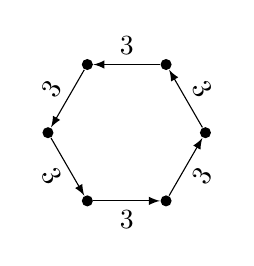
\begin{tikzpicture}
			\tikzset{vertex/.style = {shape=circle,fill,minimum size=.4em, inner sep=0pt}}
			\tikzset{edge/.style = {->,> = latex}}
			% Draw C_6
			\node[vertex] (A) at (0:1) {};
			\node[vertex] (B) at (60:1) {};
			\node[vertex] (C) at (120:1) {};
			\node[vertex] (D) at (180:1) {};
			\node[vertex] (E) at (240:1) {};
			\node[vertex] (F) at (300:1) {};
			\draw[edge] (A) to node[midway, sloped, above] {3} (B);
			\draw[edge] (B) to node[midway, sloped, above] {3} (C);
			\draw[edge] (C) to node[midway, sloped, above] {3} (D);
			\draw[edge] (D) to node[midway, sloped, below] {3} (E);
			\draw[edge] (E) to node[midway, sloped, below] {3} (F);
			\draw[edge] (F) to node[midway, sloped, below] {3} (A);
		\end{tikzpicture}
		\caption{A \(\mathbb{Z}\)-circulation on \(C_6\).}
		\label{fig:circulation_a}
	\end{subfigure}
	\begin{subfigure}{.3\textwidth}
		\centering
		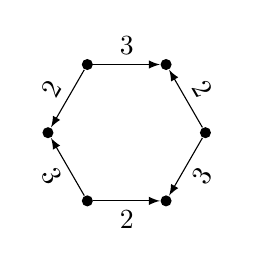
\begin{tikzpicture}
			\tikzset{vertex/.style = {shape=circle,fill,minimum size=.4em, inner sep=0pt}}
			\tikzset{edge/.style = {->,> = latex}}
			% Draw C_6
			\node[vertex] (A) at (0:1) {};
			\node[vertex] (B) at (60:1) {};
			\node[vertex] (C) at (120:1) {};
			\node[vertex] (D) at (180:1) {};
			\node[vertex] (E) at (240:1) {};
			\node[vertex] (F) at (300:1) {};
			\draw[edge] (A) to node[midway, sloped, above] {2} (B);
			\draw[edge] (C) to node[midway, sloped, above] {3} (B);
			\draw[edge] (C) to node[midway, sloped, above] {2} (D);
			\draw[edge] (E) to node[midway, sloped, below] {3} (D);
			\draw[edge] (E) to node[midway, sloped, below] {2} (F);
			\draw[edge] (A) to node[midway, sloped, below] {3} (F);
		\end{tikzpicture}
		\caption{A \(\mathbb{Z}_5\)-circulation on \(C_6\).}
		\label{fig:circulation_b}
	\end{subfigure}
	\begin{subfigure}{.3\textwidth}
		\centering
		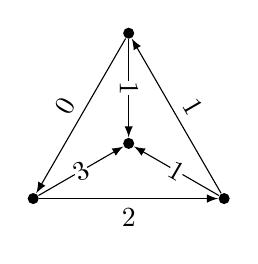
\begin{tikzpicture}
			\tikzset{vertex/.style = {shape=circle,fill,minimum size=.4em, inner sep=0pt}}
			\tikzset{edge/.style = {->,> = latex}}
			% Draw tetrahedron
			\node[vertex] (A) at ( 90:1.4) {};
			\node[vertex] (B) at (210:1.4) {};
			\node[vertex] (C) at (330:1.4) {};
			\node[vertex] (D) at (0:0) {};
			\draw[edge] (A) to node[midway, sloped, above] {0} (B);
			\draw[edge] (B) to node[midway, sloped, below] {2} (C);
			\draw[edge] (C) to node[midway, sloped, above] {1} (A);
			\draw[edge] (A) to node[midway, sloped, fill=white, inner sep=0pt] {1} (D);
			\draw[edge] (B) to node[midway, sloped, fill=white, inner sep=0pt] {3} (D);
			\draw[edge] (C) to node[midway, sloped, fill=white, inner sep=0pt] {1} (D);
		\end{tikzpicture}
		\caption{A \(\mathbb{Z}_5\)-circulation on \(K_4\).}
		\label{fig:circulation_c}
	\end{subfigure}
	\caption{Examples of circulations on graphs.}
	\label{fig:circulations}
\end{figure}

\begin{proposition} \label{prop:circulation_abelian_group}
	The set of \(H\)-circulations on \(G\) is an abelian group, with addition and negation defined pointwise, and the zero function as the identity.
\end{proposition}

\begin{proposition} \label{prop:circulation_fXX}
	Let \(f\) be an \(H\)-circulation on \(G\).
	Let \(X \subset V\).
	Then,
	\begin{equation}
		f(X, X) = 0.
	\end{equation}
\end{proposition}

\begin{proof}
	Recall that \(f(X, X)\) is the sum of \(f(\vec{e})\) over all directed edges \(\vec{e} = (e, x, y)\in \vec{E}(X, X)\).
	Note that the map \(\vec{e} = (e, x, y) \mapsto -\vec{e} = (e, y, x)\) is an involution on \(\vec{E}(X, X)\); which has no fixed points since \(\vec{E}(X, X)\) contains no loops.
	Let \(R\) be a set of representatives for the orbits of this involution.
	Then, we have
	\begin{equation}
		f(X, X) = \sum_{\vec{e} \in \vec{E}(X, X)} f(\vec{e}) = \sum_{\vec{e} \in R} f(\vec{e}) - f(-\vec{e}) = 0,
	\end{equation}
	where the last equality follows from condition~\ref{item:circulation_antisymmetry} in Definition~\ref{def:circulation}.
\end{proof}

\begin{proposition} \label{prop:circulation_fXV}
	Let \(f\) be an \(H\)-circulation on \(G\).
	Let \(X \subset V\).
	Then,
	\begin{equation}
		f(X, V) = 0.
	\end{equation}
\end{proposition}

\begin{proof}
	We have
	\begin{equation}
		f(X, V) = \sum_{x \in X} f(x, V) = 0,
	\end{equation}
	where the last equality follows from condition~\ref{item:circulation_balance} in Definition~\ref{def:circulation}.
\end{proof}

\begin{lemma} \label{lem:circulation_fXVX}
	Let \(f\) be an \(H\)-circulation on \(G\).
	Let \(X \subset V\). Then,
	\begin{equation}
		f(X, V \setminus X) = 0.
	\end{equation}
\end{lemma}
\begin{proof}
	We have
	\begin{equation}
		f(X, V \setminus X) = f(X, V) - f(X, X) = 0,
	\end{equation}
	using Propositions~\ref{prop:circulation_fXX} and~\ref{prop:circulation_fXV}.
\end{proof}

\begin{corollary} \label{cor:circulation_cut_edge}
	Let \(e\) be a cut-edge of \(G\) with endpoints \(x\) and \(y\).
	Then, \(f(e, x, y) = 0\).
\end{corollary}

\begin{proof}
	Since \(e\) is a cut-edge of \(G\) with endpoints \(x\) and \(y\),
	there exists a set \(X\) such that \(x \in X\), \(y \in V \setminus X\), and \(e\) is the only edge with one endpoint in \(X\) and the other in \(V \setminus X\).
	Then, \(\vec{E}(X, V \setminus X) = \{(e, x, y)\}\), and so, by Lemma~\ref{lem:circulation_fXVX},
	\begin{equation}
		f(e, x, y) = f(X, V \setminus X) = 0. \qedhere
	\end{equation}
\end{proof}

\begin{definition}[\(H\)-flow]
	Let \(G\) be a multigraph and let \(H\) be an abelian additive group.
	An \(H\)-circulation \(f\) on \(G\) is an \vocab{\(H\)-flow} if \(f(\vec{e}) \neq 0\) for all \(\vec{e} \in \vec{E}\).
\end{definition}

\begin{corollary} \label{cor:flow_cut_edge}
	Let \(G\) be a multigraph and let \(H\) be an abelian additive group.
	If \(G\) has a cut-edge, then it has no \(H\)-flows.
\end{corollary}

\begin{proposition}
	A multigraph \(G\) has a \(\mathbb{Z}_2\)-flow if and only if every vertex has even degree.
\end{proposition}

\begin{proof}
	Suppose \(G\) has a \(\mathbb{Z}_2\)-flow \(f\).
	Since \(f\) only takes non-zero values, \(f\) must be the constant function \(1\).
	Let \(x\) be a vertex, and let \(e_1, e_2, \ldots, e_{k}\) be the non-loop edges incident to \(x\), with other endpoints \(y_1, y_2, \ldots, y_{k}\), respectively.
	By condition~\ref{item:circulation_balance} in Definition~\ref{def:circulation}, we have in \(\mathbb{Z}_2\),
	\begin{equation}
		0 \equiv f(x, V) \equiv \sum_{i \equiv 1}^{k} f(e_i, x, y_i) \equiv \sum_{i \equiv 1}^k 1 \equiv k,
	\end{equation}
	and consequently \(k\) is even, hence the degree of \(x\) is even.
	Since \(x\) was arbitrary, every vertex of \(G\) has even degree.

	Conversely, assume that every vertex of \(G\) has even degree.
	Then, the constant function \(1\) is a \(\mathbb{Z}_2\)-flow on \(G\).
\end{proof}

\begin{proposition}
	A three-regular multigraph \(G\) has a \(\mathbb{Z}_3\) flow if and only if \(G\) is bipartite.
\end{proposition}

\begin{proof}
	Suppose \(G\) has a \(\mathbb{Z}_3\)-flow \(f\).
	Let \(x\) be a vertex, and let \(e_1, e_2, e_3\) be the edges incident to \(x\), with other endpoints \(y_1, y_2, y_3\), respectively.
	Then, we have
	\begin{equation}
		f(e_1, x, y_1) + f(e_2, x, y_2) + f(e_3, x, y_3) = 0.
	\end{equation}
	Since each of the three summands are either \(1\) or \(2\), and their sum is \(0\), they must all be equal.
	Define \(c(x)\) to be the value of \(f(e, x, y)\) for any edge \(e\) incident to \(x\), which we have just shown is well-defined.

	Note that \(c\) is a proper \(2\)-coloring of \(G\), since if \(e\) is an edge with endpoints \(x\) and \(y\), then
	\begin{equation}
		c(x) + c(y) = f(e, x, y) + f(e, y, x) = 0,
	\end{equation}
	and consequently \(c(x) \neq c(y)\).

	Conversely, assume \(G\) is bipartite.
	Let \(U\) and \(W\) be the two parts of the bipartition.
	Define \(f(e, x, y) = 1\) if \(x \in U\) and \(y \in W\),
	and \(f(e, x, y) = 2\) if \(x \in W\) and \(y \in U\).
	Then, \(f\) is a \(\mathbb{Z}_3\) flow on \(G\).
\end{proof}

\section{Flow Polynomials}

\begin{theorem}[\cite{Tutte1954}] \label{thm:flow_polynomial}
	Let \(G\) be a multigraph.
	There exists a polynomial \(P_G\)
	with integer coefficients such that,
	for any finite abelian group \(H\),
	the number of \(H\)-flows on \(G\) is \(P(|H| - 1)\).
\end{theorem}

The polynomial \(P_G\) is called the \vocab{flow polynomial} of \(G\).
Before we prove Theorem~\ref{thm:flow_polynomial}, we define the deletion and contraction of edges in a multigraph and prove lemmas about the number of flows in the resulting multigraphs.

\begin{definition}[Deletion]
	Let \(G = (V, E, r)\) be a multigraph with an edge \(e_0\).
	The multigraph \(G - e_0\) is the multigraph obtained by deleting \(e_0\) from \(G\);
	that is,
	\(G_1\) has the same vertex set as \(G\),
	has edge set \(E \setminus \{e_0\}\),
	and its incidence function \(r_1\) is the restriction of \(r\) to \(E \setminus \{e_0\}\).
\end{definition}

\begin{definition}[Contraction]
	Let \(G = (V, E, r)\) be a multigraph with an edge \(e_0\) with endpoints \(x\) and \(y\).
	Let \(z \notin V\).
	Let \(\phi \colon V \to V \setminus \{x, y\} \cup \{z\}\) be the function such that \(\phi(v) = v\) for all \(v \neq x, y\), and \(\phi(x) = \phi(y) = z\).
	The multigraph \(G / e_0\) is the multigraph obtained by contracting \(e_0\);
	that is,
	\(G_2\) has vertex set \(V \setminus \{x, y\} \cup \{z\}\),
	has edge set \(E \setminus \{e_0\}\),
	and its incidence function \(r_2\) is defined by \(\phi \circ r_1\).
\end{definition}

\begin{lemma} \label{lem:recursion_flow_polynomial}
	Let \(G\) be a multigraph with an edge \(e_0\) with distinct endpoints \(x\) and \(y\).
	Let \(H\) be a finite abelian group.
	Let \(F\), \(F_1\), and \(F_2\) be the sets of \(H\)-flows on \(G\), \(G - e_0\), and \(G / e_0\), respectively.
	Then,
	\begin{equation}
		|F| = |F_2| - |F_1|.
	\end{equation}
\end{lemma}

\begin{proof}
	Let \(z \notin V\) be the vertex obtained by contracting \(e_0\),
	and let \(\phi \colon V \to V \setminus \{x, y\} \cup \{z\}\) be the function such that \(\phi(v) = v\) for all \(v \neq x, y\), and \(\phi(x) = \phi(y) = z\).

	Let \(C_1\) be the set of \(H\)-circulations on \(G\) that are nonzero on \(E \setminus \{e_0\}\) and zero on \(e_0\).
	Let \(C_2\) be the set of \(H\)-circulations on \(G\) that are nonzero on \(E \setminus \{e_0\}\).
	This proof is divided into the proof of three claims:
	\(|F| = |C_2| - |C_1|\),
	\(|C_1| = |F_1|\), and
	\(|C_2| = |F_2|\).

	Note that \(F\) is the set of \(H\)-flows on \(G\), that is, the set of \(H\)-circulations on \(G\) that are nonzero on all edges.
	Therefore, \(F = C_2 \setminus C_1\), and so \(|F| = |C_2| - |C_1|\).

	Consider the map from \(C_1\) to \(F_1\) that sends a circulation \(f \in C_1\) to the restriction of \(f\) to \(G_1\), whose inverse is the map from \(F_1\) to \(C_1\) that sends a flow \(g \in F_1\) to the circulation that agrees with \(g\) on \(G_1\) and is zero on \(e_0\).
	Since this map has an inverse, it is a bijection, and so \(|C_1| = |F_1|\).

	Consider the map from \(C_2\) to \(F_2\) that sends a circulation \(f \in C_2\)
	to the flow \(g \in F_2\) such that, for all \(e\) with \(r_G(e) = \{u, v\}\) and \((u, v) \neq (y, x)\),
	\begin{equation}
		g(e, \phi(u), \phi(v)) = f(e, u, v).
	\end{equation}
	To check that \(g\) is indeed a flow, we need to verify that \(g\) satisfies the conditions in Definition~\ref{def:circulation}.
	By Proposition~\ref{prop:circulation_fXV} applied to \(f\) and \(X = \{x, y\}\), Condition~\ref{item:circulation_balance} for \(v = z\) is satisfied.
	All other conditions are straightforward to check.
	Finally, we claim that this is a bijection by constructing its inverse.
	Consider the map from \(F_2\) to \(C_2\) that sends a flow \(g \in F_2\)
	to the circulation \(f \in C_2\) such that,
	for all \(e \neq e_0\) with \(r_G(e) = \{u, v\}\) and \((u, v) \neq (y, x)\),
	\begin{equation}
		f(e, u, v) = g(e, \phi(u), \phi(v)),
	\end{equation}
	for all \(e \neq e_0\) with \(r_G(e) = \{y, x\}\),
	\begin{equation}
		f(e, y, x) = -g(e, z, z),
	\end{equation}
	for \(e_0\),
	\begin{equation}
		f(e_0, x, y) = - \sum_{\substack{(e, x, v) \in \vec{E}(x, V) \\ e \neq e_0}} g(e, z, \phi(v)).
	\end{equation}
	and
	\begin{equation}
		f(e_0, y, x) = \sum_{\substack{(e, x, v) \in \vec{E}(x, V) \\ e \neq e_0}} g(e, z, \phi(v)).
	\end{equation}
	It is straightforward to check that \(f\) is a circulation, that \(f\) assigns nonzero values on \(E \setminus \{e_0\}\), and that this map from \(F_2\) to \(C_2\) is the inverse of the map from \(C_2\) to \(F_2\).
	Therefore, this map is a bijection, and so \(|C_2| = |F_2|\).

	Combining the three claims, we have
	\begin{equation}
		|F| = |C_2| - |C_1| = |F_2| - |F_1|. \qedhere
	\end{equation}
\end{proof}

\begin{proof}[Proof of Theorem~\ref{thm:flow_polynomial}]
	We use induction on the number \(m\) of edges of \(G\) to prove the existence of the flow polynomial \(P_G\).

	Let \(G\) be a multigraph with \(m\) edges.
	Assume, for the induction hypothesis, that any multigraph with fewer than \(m\) edges has a flow polynomial.

	Assume that the only edges of \(G\) are loops.
	For each edge \(e\), the function \(f(e, x, x)\) can take any non-zero value in \(H\),
	and so there are \((|H| - 1)^m\) \(H\)-flows on \(G\).
	So, \(P_G(x) = x^m\) is the flow polynomial of \(G\), as desired.

	Assume that \(G\) has an edge \(e_0\) with endpoints \(x\) and \(y\).
	By induction hypothesis, the multigraphs \(G - e_0\) and \(G / e_0\) have flow polynomials \(P_{G - e_0}\) and \(P_{G / e_0}\), respectively.
	Define the flow polynomial of \(G\) as
	\begin{equation} \label{eq:flow_polynomial_recursion}
		P_G(x) = P_{G / e_0}(x) - P_{G - e_0}(x).
	\end{equation}
	By Lemma~\ref{lem:recursion_flow_polynomial}, the number of \(H\)-flows on \(G\) is \(P_{G / e_0}(|H| - 1) - P_{G - e_0}(|H| - 1) = P_G(|H| - 1)\), as desired.
\end{proof}

Equation~\eqref{eq:flow_polynomial_recursion} gives a recursive algorithm to compute the flow polynomial of a multigraph, with the base case being the flow polynomial of a multigraph with only loops.
We can also use Corollary~\ref{cor:flow_cut_edge} to claim that the flow polynomial of a multigraph with a cut-edge is the zero polynomial.

\begin{example} \label{ex:k4_flow_polynomial}
	The flow polynomial of \(K_4\) is
	\begin{equation}
		\begin{aligned}
			P_{
			\vcenter{
				\hbox{
					\begin{tikzpicture}[scale = .4, yscale = .5]
						\graph[spring layout, empty nodes, nodes={circle, fill, minimum size=3pt, inner sep=0pt}] {
						1 -- {2, 3, 4},
						2 -- {3, 4},
						3 -- 4
						};
					\end{tikzpicture}
				}
			}}
			 & =
			P_{
					\vcenter{
						\hbox{
							\begin{tikzpicture}[scale = .4, yscale = .5]
								\graph[spring layout, empty nodes, nodes={circle, fill, minimum size=3pt, inner sep=0pt}] {
								1 -- 2,
								1 --[bend right=20] 3,
								1 --[bend left=20] 3,
								2 --[bend right=20] 3,
								2 --[bend left=20] 3,
								};
							\end{tikzpicture}
						}
					}}
			-
			P_{
					\vcenter{
						\hbox{
							\begin{tikzpicture}[scale = .4, yscale = .5]
								\graph[spring layout, empty nodes, nodes={circle, fill, minimum size=3pt, inner sep=0pt}] {
								1 -- {2, 3, 4},
								2 -- {3, 4},
								};
								\draw (1) -- (2);
							\end{tikzpicture}
						}
					}}
			\\
			 & =
			P_{
					\vcenter{
						\hbox{
							\begin{tikzpicture}[scale = .4, rotate=90]
								\graph[tree layout, empty nodes, nodes={circle, fill, minimum size=3pt, inner sep=0pt}] {
								1 --[bend right=30] 3,
								1 --[bend left=30] 3,
								1 --[bend right=10] 3,
								1 --[bend left=10] 3,
								};
							\end{tikzpicture}
						}
					}
				}
			-2
			P_{
					\vcenter{
						\hbox{
							\begin{tikzpicture}[scale = .4, rotate=90]
								\graph[tree layout, empty nodes, nodes={circle, fill, minimum size=3pt, inner sep=0pt}] {
								1 --[bend right=15] 3,
								1 --[bend left=15] 3,
								2 --[bend right=15] 3,
								2 --[bend left=15] 3,
								};
							\end{tikzpicture}
						}
					}
				}
			+
			P_{
					\vcenter{
						\hbox{
							\begin{tikzpicture}[scale = .4, yscale=.5]
								\graph[spring layout, empty nodes, nodes={circle, fill, minimum size=3pt, inner sep=0pt}] {
								1 -- {2, 4} -- 3,
								};
							\end{tikzpicture}
						}
					}
				}
			\\
			 & =
			P_{
					\vcenter{
						\hbox{
							\hspace{-.5em}
							\begin{tikzpicture}[scale = .4, rotate=90]
								\graph[tree layout, empty nodes, nodes={circle, fill, minimum size=3pt, inner sep=0pt}] {
								1 --[loop, out=0, in=60, looseness=10] 1,
								1 --[loop, out=120, in=180, looseness=10] 1,
								1 --[loop, out=240, in=300, looseness=10] 1,
								};
							\end{tikzpicture}
						}
					}
				}
			-
			P_{
					\vcenter{
						\hbox{
							\begin{tikzpicture}[scale = .4, rotate=90]
								\graph[tree layout, empty nodes, nodes={circle, fill, minimum size=3pt, inner sep=0pt}] {
								1 --[bend right=30] 3,
								1 --[bend left=30] 3,
								1 -- 3,
								};
							\end{tikzpicture}
						}
					}
				}
			-2
			P_{
					\vcenter{
						\hbox{
							\hspace{-.7em}
							\begin{tikzpicture}[scale = .4, rotate=90]
								\graph[tree layout, empty nodes, nodes={circle, fill, minimum size=3pt, inner sep=0pt}] {
								1 --[loop, in=135, out=60, looseness=10] 1,
								1 --[bend right=20] 2,
								1 --[bend left=20] 2,
								};
							\end{tikzpicture}
						}
					}
				}
			+2\underbrace{P_{
			\vcenter{
				\hbox{
					\begin{tikzpicture}[scale = .4, rotate=90]
						\graph[tree layout, empty nodes, nodes={circle, fill, minimum size=3pt, inner sep=0pt}] {
						1 -- 2,
						2 --[bend right=20] 3,
						2 --[bend left=20] 3,
						};
					\end{tikzpicture}
				}
			}
			}}_{=0}
			+
			P_{
					\vcenter{
						\hbox{
							\begin{tikzpicture}[scale = .4, yscale=.5]
								\graph[spring layout, empty nodes, nodes={circle, fill, minimum size=3pt, inner sep=0pt}] {
									1 -- 2 -- 3 -- 1,
								};
							\end{tikzpicture}
						}
					}
				}
			-
			\underbrace{P_{
					\vcenter{
						\hbox{
							\begin{tikzpicture}[scale = .3, rotate=90]
								\graph[tree layout, empty nodes, nodes={circle, fill, minimum size=3pt, inner sep=0pt}] {
									1 -- 2 -- 3 -- 4,
								};
							\end{tikzpicture}
						}
					}
				}}_{=0}
			\\
			 & =
			P_{
					\vcenter{
						\hbox{
							\hspace{-.5em}
							\begin{tikzpicture}[scale = .4, rotate=90]
								\graph[tree layout, empty nodes, nodes={circle, fill, minimum size=3pt, inner sep=0pt}] {
								1 --[loop, out=0, in=60, looseness=10] 1,
								1 --[loop, out=120, in=180, looseness=10] 1,
								1 --[loop, out=240, in=300, looseness=10] 1,
								};
							\end{tikzpicture}
						}
					}
				}
			-
			P_{
					\vcenter{
						\hbox{
							\hspace{-.7em}
							\begin{tikzpicture}[scale = .4, rotate=-37]
								\graph[tree layout, empty nodes, nodes={circle, fill, minimum size=3pt, inner sep=0pt}] {
								1 --[loop, out=0, in=60, looseness=10] 1,
								1 --[loop, out=180, in=240, looseness=10] 1,
								};
							\end{tikzpicture}
						}
					}
				}
			+
			P_{
					\vcenter{
						\hbox{
							\begin{tikzpicture}[scale = .4, rotate=90]
								\graph[tree layout, empty nodes, nodes={circle, fill, minimum size=3pt, inner sep=0pt}] {
								1 --[bend right=30] 3,
								1 --[bend left=30] 3,
								};
							\end{tikzpicture}
						}
					}
				}
			-2
			P_{
					\vcenter{
						\hbox{
							\hspace{-.7em}
							\begin{tikzpicture}[scale = .4, rotate=-37]
								\graph[tree layout, empty nodes, nodes={circle, fill, minimum size=3pt, inner sep=0pt}] {
								1 --[loop, out=0, in=60, looseness=10] 1,
								1 --[loop, out=180, in=240, looseness=10] 1,
								};
							\end{tikzpicture}
						}
					}
				}
			+2
			\underbrace{P_{
					\vcenter{
						\hbox{
							\hspace{-.7em}
							\begin{tikzpicture}[scale = .4, rotate=90]
								\graph[tree layout, empty nodes, nodes={circle, fill, minimum size=3pt, inner sep=0pt}] {
								1 --[loop, in=135, out=60, looseness=10] 1,
								1 -- 2,
								};
							\end{tikzpicture}
						}
					}
				}}_{=0}
			+
			P_{
					\vcenter{
						\hbox{
							\begin{tikzpicture}[scale = .4, rotate=90]
								\graph[tree layout, empty nodes, nodes={circle, fill, minimum size=3pt, inner sep=0pt}] {
								1 --[bend right=30] 3,
								1 --[bend left=30] 3,
								};
							\end{tikzpicture}
						}
					}
				}
			-
			\underbrace{P_{
				\vcenter{
					\hbox{
						\begin{tikzpicture}[scale = .4, rotate=90]
							\graph[tree layout, empty nodes, nodes={circle, fill, minimum size=3pt, inner sep=0pt}] {
								1 -- 2 -- 3,
							};
						\end{tikzpicture}
					}
				}
			}}_{=0}
			\\
			 & =
			P_{
					\vcenter{
						\hbox{
							\hspace{-.5em}
							\begin{tikzpicture}[scale = .4, rotate=90]
								\graph[tree layout, empty nodes, nodes={circle, fill, minimum size=3pt, inner sep=0pt}] {
								1 --[loop, out=0, in=60, looseness=10] 1,
								1 --[loop, out=120, in=180, looseness=10] 1,
								1 --[loop, out=240, in=300, looseness=10] 1,
								};
							\end{tikzpicture}
						}
					}
				}
			-
			3P_{
					\vcenter{
						\hbox{
							\hspace{-.7em}
							\begin{tikzpicture}[scale = .4, rotate=-37]
								\graph[tree layout, empty nodes, nodes={circle, fill, minimum size=3pt, inner sep=0pt}] {
								1 --[loop, out=0, in=60, looseness=10] 1,
								1 --[loop, out=180, in=240, looseness=10] 1,
								};
							\end{tikzpicture}
						}
					}
				}
			+
			2P_{
					\vcenter{
						\hbox{
							\begin{tikzpicture}[scale = .4, rotate=-37]
								\graph[tree layout, empty nodes, nodes={circle, fill, minimum size=3pt, inner sep=0pt}] {
									1 --[loop, out=0, in=60, looseness=10] 1,
								};
							\end{tikzpicture}
						}
					}
				}
				-
				2\underbrace{P_{
					\vcenter{
						\hbox{
							\begin{tikzpicture}[scale = .4, rotate=90]
								\graph[tree layout, empty nodes, nodes={circle, fill, minimum size=3pt, inner sep=0pt}] {
								1 -- 2,
								};
							\end{tikzpicture}
						}
					}
				}}_{=0}
			\\
			 & =
			x^3 - 3x^2 + 2x.
		\end{aligned}
	\end{equation}

	In particular, \(P_{K_4}(1) = 0\), which implies that \(K_4\) has no \(\mathbb{Z}_2\)-flows.
	This is consistent with the fact that \(K_4\) does not have all vertices of even degree.
	Similarly, \(P_{K_4}(2) = 0\), which implies that \(K_4\) has no \(\mathbb{Z}_3\)-flows.
	This is consistent with the fact that \(K_4\) is not bipartite.
	Similarly, \(P_{K_4}(3) = 6\), which implies that \(K_4\) has \(6\) \(\mathbb{Z}_4\)-flows, as well as \(6\) \((\mathbb{Z}_2 \times \mathbb{Z}_2)\)-flows.
\end{example}

As exemplified, the algorithm induced by the proof of Tutte's theorem takes exponential time.
There's a line of research in studying properties and algorithms for flow polynomials.

\section{Flow Number and Existence of Flows}

\begin{definition}[Flow number]
	A \(\mathbb{Z}\)-flow on a multigraph \(G\) is a \vocab{\(k\)-flow} if \(|f(\vec{e})| \leq k\) for all \(\vec{e} \in \vec{E}\).
	The smallest \(k\) for which \(G\) has a \(k\)-flow is the \vocab{flow number} of \(G\), denoted by \(\phi(G)\).
\end{definition}

It is worth noting that any \(k\)-flow can be seen as a \(\mathbb{Z}_k\)-flow,
while the converse is not necessarily true.

\begin{example}
	By Example~\ref{ex:k4_flow_polynomial}, \(K_4\) has no \(\mathbb{Z}_2\)-flows or \(\mathbb{Z}_3\)-flows,
	and consequently \(K_4\) has no \(2\)-flows or \(3\)-flows.
	Figure~\ref{fig:k4_4_flow} shows a \(4\)-flow on \(K_4\).
	Therefore, the flow number of \(K_4\) is \(\phi(K_4) = 4\).
\end{example}

\begin{figure}[htbp]
	\centering
	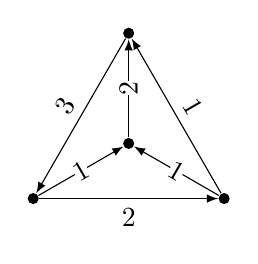
\begin{tikzpicture}
		\tikzset{vertex/.style = {shape=circle,fill,minimum size=.4em, inner sep=0pt}}
		\tikzset{edge/.style = {->,> = latex}}
		% Draw tetrahedron
		\node[vertex] (A) at ( 90:1.4) {};
		\node[vertex] (B) at (210:1.4) {};
		\node[vertex] (C) at (330:1.4) {};
		\node[vertex] (D) at (0:0) {};
		\draw[edge] (A) to node[midway, sloped, above] {3} (B);
		\draw[edge] (B) to node[midway, sloped, below] {2} (C);
		\draw[edge] (C) to node[midway, sloped, above] {1} (A);
		\draw[edge] (D) to node[midway, sloped, fill=white, inner sep=0pt] {2} (A);
		\draw[edge] (B) to node[midway, sloped, fill=white, inner sep=0pt] {1} (D);
		\draw[edge] (C) to node[midway, sloped, fill=white, inner sep=0pt] {1} (D);
	\end{tikzpicture}
	\caption{A \(4\)-flow on \(K_4\).}
	\label{fig:k4_4_flow}
\end{figure}


\begin{theorem}[Tutte (1950)] \label{thm:k-flow-Zk-flow}
	A multigraph \(G\) has a \(k\)-flow if, and only if, \(G\) has a \(\mathbb{Z}_k\)-flow.
\end{theorem}

\begin{proof}
	By mapping \(\mathbb{Z}\) onto \(\mathbb{Z}_k\), the existence of a \(k\)-flow implies the existence of a \(\mathbb{Z}_k\)-flow. It remains to show the converse.

	Assume, without loss of generality, that \(G\) has no loops.
	Let \(g \colon \vec{E} \to \mathbb{Z}_k\) be a \(\mathbb{Z}_k\)-flow on \(G\).

	Let \(f \colon \vec{E} \to \mathbb{Z}\) be a function such that, for all \(\vec{e} \in \vec{E}\),
	\begin{enumerate}
		\item \(0 < |f(\vec{e})| < k\),
		\label{item:k-flow-Zk-flow-a}
		\item \(f(\vec{e}) = -f(\cev{e})\),
		\label{item:k-flow-Zk-flow-b}
		\item \(f(\vec{e}) \equiv g(\vec{e}) \pmod{k}\),
		\label{item:k-flow-Zk-flow-c}
	\end{enumerate}
	for which 
	\begin{equation}
		K(f) = \sum_{x \in V} |f(x, V)|
	\end{equation}
	is minimized.

	It is straightforward to check that such function \(f\) exists.

	Assume, by the sake of contradiction, that \(K(f) > 0\).

	Since item~\ref{item:k-flow-Zk-flow-b} is satisfied, we have that
	\begin{equation}
		\sum_{x \in V} f(x, V) = 0.
	\end{equation}
	Therefore, there must be a vertex \(x\) such that \(f(x, V) > 0\).
	Let \(X\) be the set of vertices \(y\) reachable from \(x\) by a directed path of edges with positive flow;
	that is, \(X\) is the set of vertices \(y\) such that there exists a sequence of vertices \(x = x_0, x_1, \ldots, x_k = y\) and edges \(\vec{e}_1 = (e_1, x_0, x_1), \ldots, \vec{e}_k = (e_k, x_{k-1}, x_k)\) such that \(f(\vec{e}_i) > 0\) for all \(i\).

	Note that, for any edge \(e\) with endpoints \(v \in X\) and \(y \in V \setminus X\), we have \(f(e, v, y) < 0\), since otherwise \(y\) would be reachable from \(x\) by a directed path of edges with positive flow.
	Therefore,
	for all \(v \in X\),
	\begin{equation} \label{eq:k-flow-Zk-flow:fvV-X}
		f(v, V \setminus X) \leq 0.
	\end{equation}
	In particular, Equation~\eqref{eq:k-flow-Zk-flow:fvV-X} with \(v = x\) implies that
	\(f(x, V \setminus X) \leq 0\).
	Since \(f(x, V) > 0\), we have 
	\begin{equation} \label{eq:k-flow-Zk-flow:fxV-X}
		f(x, X \setminus \{x\}) > 0.
	\end{equation}
	Moreover, summing Equation~\eqref{eq:k-flow-Zk-flow:fvV-X} for all \(v \in X \setminus \{x\}\) gives
	\begin{equation} \label{eq:k-flow-Zk-flow:sumfX-xV-X}
		f(X \setminus \{x\}, V \setminus X) \leq 0.
	\end{equation}

	Finally, from Equations~\eqref{eq:k-flow-Zk-flow:fxV-X}
	and \eqref{eq:k-flow-Zk-flow:sumfX-xV-X}, we have
	\begin{align*}
		\sum_{v \in X \setminus \{x\}} f(v, V)
		& = f(X \setminus \{x\}, V) \\
		& = f(X \setminus \{x\}, V \setminus X) + f(X \setminus \{x\}, x) + f(X \setminus \{x\}, X \setminus \{x\}) < 0,
	\end{align*}
	and, consequently, there exists \(x' \in X \setminus \{x\}\) such that \(f(x', V) < 0\).

	Since \(x' \in X\), there exists a directed path \(x = x_0, x_1, \ldots, x_k = x'\) with edges \(\vec{e}_1 = (e_1, x_0, x_1), \ldots, \vec{e}_k = (e_k, x_{k-1}, x_k)\) such that \(f(\vec{e}_i) > 0\) for all \(i\).
	Define \(f'\) as the function such that, for all \(\vec{e} = (e, u, v) \in \vec{E}\),
	\begin{equation}
		f'(e, u, v) =
		\begin{cases}
			f(e, u, v) - k & \text{if } (e, u, v) = (e, x_{i-1}, x_i) \text{ for some } i, \\
			f(e, u, v) + k & \text{if } (e, u, v) = (e, x_{i}, x_{i-1}) \text{ for some } i, \\
			f(e, u, v) & \text{otherwise}.
		\end{cases}
	\end{equation}

	It is straightforward to check that \(f'\) satisfies conditions \ref{item:k-flow-Zk-flow-a}, \ref{item:k-flow-Zk-flow-b}, and \ref{item:k-flow-Zk-flow-c}.

	Note that, for all \(v \notin \{x, x'\}\), we have \(f'(v, V) = f(v, V)\).
	Note that \(f(x, V) > 0\) and \(f(x, V) \equiv g(x, V) \equiv 0 \pmod{k}\), hence \(f(x, V) \geq k\), and consequently
	\begin{equation}
		f'(x, V) = f(x, V) - k \geq 0,
	\end{equation}
	which implies that \(|f(x, V)| > |f'(x, V)|\).
	By a similar argument, \(|f(x', V)| > |f'(x', V)|\).
	Therefore,
	\begin{equation}
		K(f) = \sum_{v \in V} |f(v, V)| > \sum_{v \in V} |f'(v, V)| = K(f'),
	\end{equation}
	which contradicts the minimality of \(K(f)\).

	Therefore, \(K(f) = 0\), and so \(f\) is a \(k\)-flow on \(G\), as desired.
\end{proof}

Let's try to compute the flow number of complete graphs \(K_n\).
If \(n > 1\) is an odd number, then \(K_n\) is an Eulerian graph, and so \(\phi(K_n) = 2\).
The flow number of \(K_2\) doesn't exist, since \(K_2\) has a cut-edge.
In Example~\ref{ex:k4_flow_polynomial}, we computed that \(\phi(K_4) = 4\).

Note that, if \(G_1\) and \(G_2\) are edge-disjoint, then a \(k\)-flow on \(G_1\) and a \(k\)-flow on \(G_2\) can be combined to form a \(k\)-flow on \(G_1 \cup G_2\); hence
\begin{equation}
	\phi(G_1 \cup G_2) \leq \max\{\phi(G_1), \phi(G_2)\}.
\end{equation}

\begin{proposition}
	The flow number of a complete graph \(K_6\) is \(3\).
\end{proposition}

\begin{proof}
	Split \(K_6\) into two copies of \(K_3\), and one copy of \(K_{3, 3}\), which have flow numbers \(2\), \(2\), and \(3\), respectively.
	Therefore, \(\phi(K_6) \leq 3\).
	With \(\phi(K_6) > 2\), it follows that \(\phi(K_6) = 3\).
\end{proof}

\begin{theorem}
	Let \(n \geq 6\) be an even integers.
	Then, \(\phi(K_n) = 3\).
\end{theorem}

\begin{proof}
	Induction on \(n\).
\end{proof}

\begin{proposition}
	The Petersen graph has flow number \(5\).
\end{proposition}

\begin{figure}
	% The Petersen graph:
	\centering
	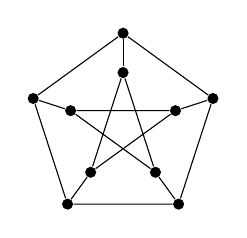
\begin{tikzpicture}[scale = .5]
		\tikzset{vertex/.style = {shape=circle,fill,minimum size=.4em, inner sep=0pt}}
		% Draw Petersen graph
		\node[vertex] (A) at ( 90:1.4) {};
		\node[vertex] (B) at (162:1.4) {};
		\node[vertex] (C) at (234:1.4) {};
		\node[vertex] (D) at (306:1.4) {};
		\node[vertex] (E) at (18:1.4) {};
		\node[vertex] (F) at (90:2.4) {};
		\node[vertex] (G) at (162:2.4) {};
		\node[vertex] (H) at (234:2.4) {};
		\node[vertex] (I) at (306:2.4) {};
		\node[vertex] (J) at (18:2.4) {};
		\draw (A) -- (C) -- (E) -- (B) -- (D) -- (A);
		\draw (F) -- (G) -- (H) -- (I) -- (J) -- (F);
		\draw (F) -- (A);
		\draw (G) -- (B);
		\draw (H) -- (C);
		\draw (I) -- (D);
		\draw (J) -- (E);	
	\end{tikzpicture}
\end{figure}

\begin{conjecture}[Tutte's \(5\)-flow conjecture (1954)]
	Every bridgeless multigraph has a \(5\)-flow.
\end{conjecture}

\begin{conjecture}[Tutte's \(4\)-flow conjecture (1966)]
	Every bridgeless multigraph without a Petersen minor has a \(4\)-flow.	
\end{conjecture}

\begin{conjecture}[Tutte's \(3\)-flow conjecture (1972)]
	Every multigraph without an edge cut of size \(1\) or \(3\) has a \(3\)-flow.
\end{conjecture}

These conjectures were thought to help in proving the Four-Color Theorem.
All of these conjectures are true for planar graphs.

We will prove an weaker version of Tutte's \(5\)-flow conjecture.

\begin{theorem}[\(6\)-flow theorem, Seymour (1981)]
	Every bridgeless multigraph has a \(6\)-flow.
\end{theorem}

\begin{proof}
	Let \(G\) be a bridgeless multigraph.
	Assume, without loss of generality, that \(G\) has no loops.

	By Menger's theorem,
	since \(G\) is bridgeless, that is, \(G\) is \(2\)-edge-connected,
	for all \(u, v \in V\),
	there are two edge-disjoint paths from \(u\) to \(v\).
	By taking the union of these paths,
	for all \(u, v \in V\),
	there exists an even connected subgraph \(G_{u, v} = (V_{u, v}, E_{u, v})\) of \(G\) such that \(u, v \in V_{u, v}\).

	Let \(H_0\) be a subgraph of \(G\) with one vertex and no edges.
	Assume disjoint even connected subgraphs \(H_0, \dots, H_{i-1}\) have been defined, together with edge sets \(F_1, \dots, F_{i-1}\) such that, for each \(j < i\),
	\(F_j\) contains exactly one or two edges joining \(V(H_j)\) to \(\bigcup_{t = 0}^{j-1} V(H_t)\).
	Then, \(H^{i-1}\) with vertex set \(\bigcup_{t = 0}^{i-1} V(H_t)\) and edge set
	\begin{equation}
		\medmuskip=20mu
		\bigcup_{t = 0}^{i-1} E(H_t) \cup \bigcup_{t = 1}^{i-1} F_t
	\end{equation}
	is connected.

	If \(V(H^{i-1}) = V\), then we stop. Set \(s = i - 1\).
	Otherwise,
	let \(X_i\) be a smallest nonempty subset of \(V \setminus V(H^{i-1})\) such that the number of edges from \(X_i\) to \(V(G) \setminus (X_i \cup V(H^{i-1}))\) is less or equal to \(1\); that is,
	\begin{equation}
		\left| E\left(X_i, V(G) \setminus (X_i \cup V(H^{i-1}))\right) \right| \leq 1.
	\end{equation}
	Note that such \(X_i\) exists because \(V(G) \setminus V(H^{i-1})\) is a candidate.

	Note that there exist edges joining \(X_i\) to \(V(H^{i-1})\) since \(G\) is bridgeless.

	Assume, by the sake of contradiciton, that the subgraph induced by \(X_i\) has a bridge.
	Then, there exist two disjoint nonempty subsets \(A, B \subseteq X_i\), with \(A \cup B = X_i\), such that there is at most \(1\) edge between \(A\) and \(B\); that is,
	\begin{equation}
		\left| E(A, B) \right| \leq 1.
	\end{equation}
	Then, either \(A\) or \(B\) is a smaller nonempty subset of \(V \setminus V(H^{i-1})\) such that the number of edges from \(A\) to \(V(G) \setminus (A \cup V(H^{i-1}))\) is less or equal to \(1\), which contradicts the minimality of \(X_i\).
	Therefore, the subgraph induced by \(X_i\) is bridgeless, and consequently connected.

	If \(|E(X_i, V(H^{i-1}))| \geq 2\), 
	then we choose any two such edges to be \(F_i\).
	Let \(x, y\) be the two endpoins in \(X_i\) of the edges in \(F_i\).
	Let \(H_i = G_{x, y}\).

	Otherwise, if \(|E(X_i, V(H^{i-1}))| = 1\),
	then we choose this edge to be \(F_i\),
	and let \(x\) be the endpoint in \(X_i\) of the edge in \(F_i\).
	Let \(H_i = G_{x}\).
	Note that, since \(G\) is bridgeless,
	there exists an edge joining \(X_i\) to \(V(G) \setminus (X_i \cup V(H^{i-1}))\).
	Therefore,
	\begin{equation}
		|E(X_i, V(G) \setminus (X_i \cup V(H^{i-1})))| = 1.
	\end{equation}

	Therefore,
	we have a sequence of even connected subgraphs \(H_0, \dots, H_s\) of \(G\),
	and a sequence of edge sets \(F_1, \dots, F_s\),
	such that
	\begin{gather}
		\bigcup_{t = 0}^{s} V(H_t) = V \\
		F_t \subseteq E(H_t) \text{ for all } t \in \{1, \dots, s\}, \\
		|F_t| \in \{1, 2\} \text{ for all } t \in \{1, \dots, s\}, \\
	\end{gather}

	We define an \(\mathbb{Z}_3\)-circulation \(f\) by reverse induction.
	We define \(f_s\) on \(G\) as follows.
	For each edge \(e \notin E(H^{s})\),
	let \(C_e\) be a directed cycle in \(H^{s} + e\) containing \(e\).
	which is possible because \(H^{s}\) is connected.
	Let \(f_{s, e}\) be an \(\mathbb{Z}_3\) circulation on \(G\) by letting \(f_{s, e}\) be \(1\) on \(\vec{E}(C_e)\), \(-1\) on \(\cev{E}(C_e)\), and \(0\) on all other edges.
	Let \(f_s\) be the sum of all \(f_{s, e}\) over all \(e \notin E(H^{s})\).
	Hence, \(f_s\) is nonzero on all edges in \(E(G) \setminus E(H^{s})\).

	Assume \(f_s, f_{s-1}, \dots, f_{i}\) are \(\mathbb{Z}_3\)-circulations on \(G\) such that \(f_i\) is nonzero on
	\begin{equation}
		(E(G) \setminus E(H^{s})) \cup \bigcup_{t = i+1}^{s} F_t.
	\end{equation}

	Suppose that \(|F_i| = 1\).
	Let \(e\) be the only edge in \(F_i\).
	Then, by definition of the procedure, we have
	\begin{gather}
		|E(X_i, H^{(i-1)})| = 1, \\
		|E(X_i, V(G) \setminus (X_i \cup V(H^{(i-1)})))| = 1.
	\end{gather}
	Let \(e'\) be the edge in \(E(X_i, V(G) \setminus (X_i \cup V(H^{i-1})))\).

	Note that \(e' \notin H^{i}\).
	Therefore, \(e' \notin F_k\) for all \(k \in \{1, \dots, i\}\), and \(e' \notin H_k\) for all \(k \in \{1, \dots, i\}\).

	Note that \(e'\) is a bridge of \(G[V(G) \setminus V(H^{i-1})]\).
	Any \(H_k\) with \(k \in \{i+1, \dots, s\}\) is contained in \(G[V(G) \setminus V(H^{i-1})]\) as well.
	If \(e' \in E(H_k)\), then \(e'\) is a bridge of \(H_k\), that is, there exists a cut \((A, B)\) of \(H_k\) such that \(e'\) is the only edge joining \(A\) to \(B\).
	However, this contradicts the fact that the sum of the degrees of \(H_k[A]\) is even.
	Therefore, \(e' \notin E(H_k)\) for all \(k \in \{i+1, \dots, s\}\).

	Since \(e'\) is not in any \(H_k\) with \(k \in \{1, \dots, s\}\),
	and \(e'\) is not in any \(F_k\) with \(k \in \{1, \dots, i\}\),
	it follows that \(f_i(e')\) is nonzero.
	Since \(f_i(e') \neq 0\) and \(0 = F(X_i, V(G) \setminus (X_i \cup V(H^{i-1}))) = f_i(e') + f_i(e)\), it follows that \(f_i(e)\) is nonzero.
	Let \(f_{i-1} = f_i\).

	Now, suppose that \(|F_i| = 2\).
	Let \(e_1, e_2\) be the two edges in \(F_i\).
	Let \(C\) be a directed cycle on \(H^{i}\) containing \(e_1\) and \(e_2\).
	Let \(f_c\) be a \(\mathbb{Z}_3\)-circulation that sends \(1\) on \(\vec{E}(C)\), \(-1\) on \(\cev{E}(C)\), and \(0\) on all other edges.
	Among \(f_i\), \(f_i + f_c\), and \(f_i + 2 f_c\), at most one is zero on \(e_1\), and at most one is zero on \(e_2\).
	Let \(f_{i-1}\) be the one that is nonzero on both \(e_1\) and \(e_2\).

	By induction, we have defined a sequence of \(\mathbb{Z}_3\)-circulations \(f_1, \dots, f_s\) on \(G\) with the desired properties.
	In particular, \(f_1\) is a \(\mathbb{Z}_3\)-circulation on \(G\) that is nonzero on all edges 
	\begin{equation}
		E(G) \setminus E(H^{s}) = E(G) \setminus E(H^{s}) \cup \bigcup_{t = 1}^{s} F_t.
	\end{equation}
\end{proof}